% !TeX spellcheck = en_GB
\chapter{Optimal Estimation Retrieval Algorithm} %Section - 1.2
\label{ch:retrieval}
Since 2006, with the launch of CloudSats Cloud Profiling Radar (CPR) a global estimation of snowfall can be done. Several studies, such as \cite{kulie_utilizing_2009} have shown that estimated snowfall values depend heavily upon assumed snowflake microphysical properties.
%\textcolor{red}{Steve had some insertions but no comments.}
%depending on the retrieval assumption, snowfall estimation can give the same values for different a priori guess, e.g. snowflake microphysical properties. 
%Introducing information from snow microphysics will reduce the non-uniqueness in optimal estimation radar retrieval schemes. 
%This can be done by using the temperature at a lower level as a priori as the CloudSat retrieval does.  
%\\
\cite{wood_microphysical_2015} showed that a refinement of the CloudSat snowfall retrieval algorithm can be done by using snowflake models. 
%\textcolor{red}{That was Steves comment which is exactly what I wrote? "
This study was based on data from the Canadian CloudSat-CALIPSO Validation Project \citep[C3VP,][]{hudak_canadian_2006}, where they concentrated on cold season clouds and precipitation.
%"} 
\\
\noindent In an attempt to reduce the non-uniquness of the problem, \cite{wood_microphysical_2015} used the a priori knowledge of snowfall microphysics and temperature (from ground-based observations) to refine the forward-model assumptions for the CloudSat snowfall retrieval scheme. 
%\textcolor{red}{Steve: "They also used a temperature to introduce a priori information on particle size into the retrieval scheme. " Me: They did? So by introducing a temp they estimate the particle size?}
Results from this scheme showed a good agreement with reported values observed at meteorological measurement sites. \\
Model estimates have proven, how useful the estimation retrieval can be to verify ground-based radar snowfall measurements \citep{norin_intercomparison_2015}.
Although the retrieval has obviously been improved the estimation algorithm, can still lead to uncertainties in the retrievals of up to \SIrange{140}{200}{\percent} \citep{wood_estimation_2011}. 
\\
% \noindent The snowfall retrieval assumes an exponential particle size distribution (PSD)
% \begin{align}
% 	N(D) = N_{0} exp(-\lambda D).
% 	\label{eq:PSD}
% \end{align} 
% $\lambda$ represents here the PSD slope parameter and $N_{0}$ the number density. 
% %$D$ is the particle maximum dimension evaluated from the MASC. 
% \\
% The optimal estimation technique is based on Gaussian statistics. Minimizing the scalar cost function, $\Phi$ for the snowfall properties, $x$ by; 
% \begin{equation}
% \begin{split}
% \Phi(x,y,a) = &(y- F(x))^T \mathbf{S}_y^{-1} (\mathbf{y}-F(\mathbf{x})) \\
% &+(x-a)^T \mathbf{S}_{a}^{-1} (x-a)
% \end{split} \label{eq:scalar_cost_fct}
% \end{equation}
% where, $x$, vector of retrieved snowfall properties (slope parameter and number density); $y$, vector of observation (MRR reflectivity) ; $a$, vector of the a priori guess (temperature dependent); $F$, forward model; $\mathbf{S}_a$, a priori error covariance matrix; $\mathbf{S}_y$, measurement error covariance matrix.
% \\
\cite{cooper_variational_2017} developed a technique to combine MRR, MASC, and PiP information into a common retrieval framework. Specifically, estimates of snowflake microphysical properties from the MRR are used as the a priori term in the optimal-estimation retrieval scheme. The usage of either MASC\,/\,PiP or MRR fall-speed can show which a priori guess in the retrieval gives the more accurate retrieved snowfall rate at the ground. \\
The difference between the retrieval and the snow gauge observations was \SI{-18}{\percent} when applied to data from Barrow, Alaska.\\
\cite{cooper_variational_2017} also showed that the retrieval is sensitive to habit and fall speed. The installation of a MRR, MASC, and PIP should help to adjust the particle models for graupels and rimed particles which are often observed at Haukeliseter. 

\section{Present snow}\label{sec:pre_snow}
%\item surface temperature \SI{< 2}{\celsius}
%\item follows \Cref{fig:MRR_sfcT}
% %%% image surface temperature and MRR %%%%%%%%%%%%%%%%%%%%%%%%%%%%%%%%%%%%%
% !TeX spellcheck = en_GB
\begin{figure}[t!]
	\centering
	%    \begin{subfigure}[b]{\textwidth}
	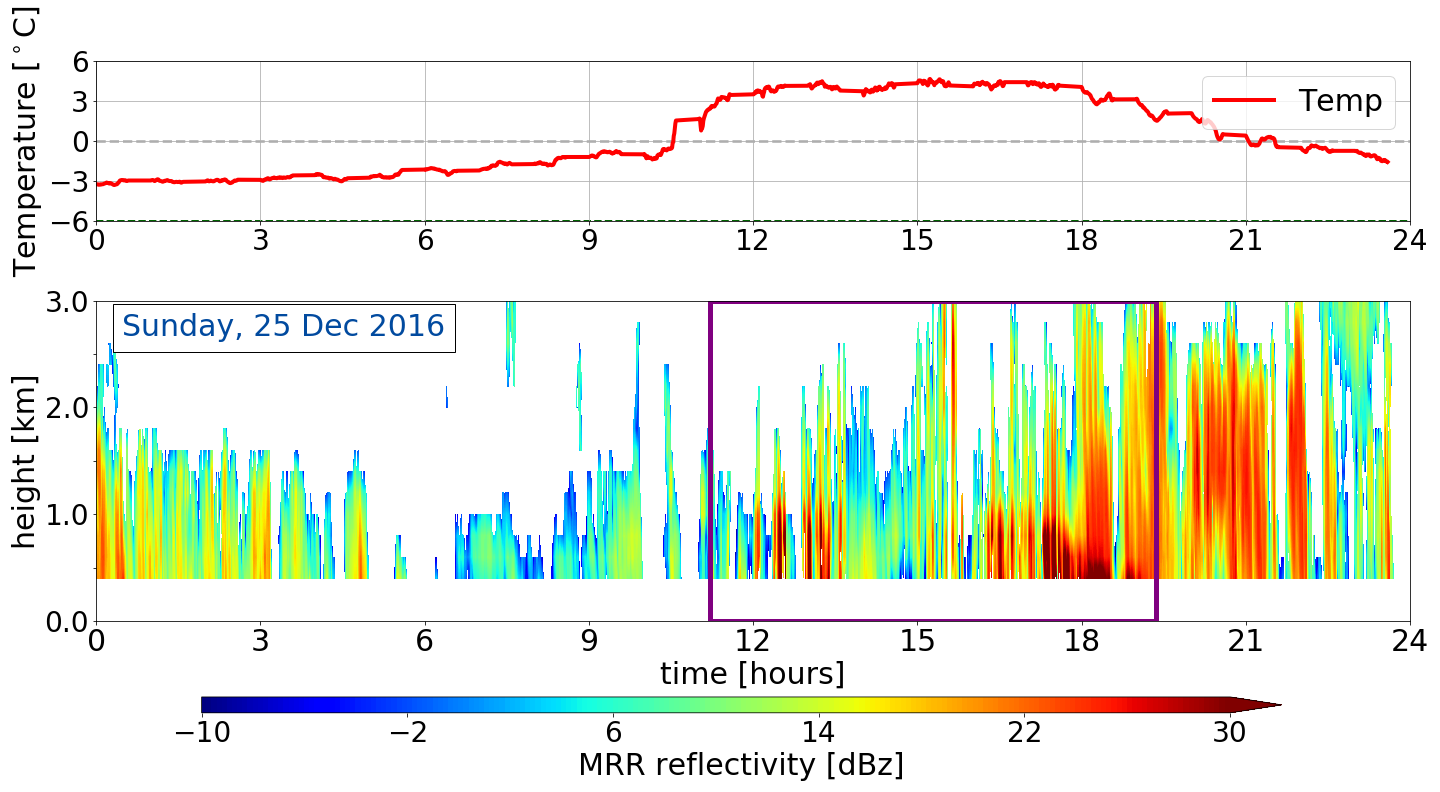
\includegraphics[width=\textwidth]{./fig_MRR/MRR_sfcT_20161225}
	%	\end{subfigure}
	\caption{A priori temperature dependence within the optimal estimation retrieval for an all day precipitation event on \SI{25}{\dec}. The upper panel shows the surface a priori guess, $T_{ap}$, measured at the Haukeliseter site. The lower panel presents the reflectivity measure by the MRR. Additionally, indicates the purple frame the time, where the MRR reflectivity was larger than \SI{-10}{\dB Z} and surface temperatures less than \SI{2}{\celsius} }\label{fig:MRR_sfcT}
\end{figure}
%%%%%%%%%%%%%%%%%%%%%%%%%%%%%%%%%%%%%%%%%%%%%%%%%%%%%%%%%%%%%%%%%%%%%%%%%%
To achieve vertical profiles of snowfall from MRR different steps and assumptions are done in the snowfall retrieval. From the lowest level, the snowfall rate at the surface can be estimated. The retrieval is only performed for profiles, which are likely to have observed snow. To obtain the likelihood of present snow a reflectivity threshold of \SI{- 15}{\decibel Z} is used. This threshold is similar to the one used in \cite{wood_level_2013}, where it states that light liquid precipitation is related to \SI{- 10}{\decibel Z} \textcolor{red}{citation here}. \cite{wood_estimation_2011} compared the reflectivities in the lowest bin and adjacent bin and found, that the reflectivity above \SI{-15}{\dB Z} are not influenced by ground clutter.
\newline
Since the MRR measures above \SI{300}{\metre} and only temperature measurements at the surface exists, a priori temperature ($T_{ap}$) is assumed to be similar to the observed near-surface air temperature. Using a moist adiabatic lapse rate of $dT/dz = \SI{5}{\kelvin\per\km}$ gives $T_{ap}$ in each layer. Temperature measurements above \SI{2}{\celsius} \textcolor{red}{read up reference Liu (2008), \cite{wood_level_2013}} are neglected and assumed to be present liquid precipitation. 
The purple line in \Cref{fig:MRR_sfcT} represents the time frame during \SI{25}{\dec}, where the MRR measures reflectivity above \SI{- 15}{\decibel Z}, and a priori temperature passes the \SI{2}{\celsius} limit at the surface.  


\section{Size distribution} \label{sec:size_dist}
To determine the snowfall rate at the surface an exponential particle size distribution (PSD) is used. 
\begin{align}
	N(D) & = N_{0} \exp\left(-\lambda D\right) \qquad [ \SI{}{\per\cubic\metre\per\mm} ] \label{eq:num_dens}
\end{align}
where $\lambda$ represents the PSD slope parameter and $N_{0}$ the number density. $D$ is the particle maximum dimension evaluated from the 2D-scattering model for hexagonal prism shaped particles at \SI{24}{\giga\Hz} (see \Cref{app:scat_scheme}).
%exponential particle size distribution (PSD) \\
%	$$ \qquad \text{$D$ from B6 scattering model}$$
%	$$\lambda = 10^{perturbuation}$$ %\\
%   %$$N_0 = 10^{perturbation}$$
%The slope parameter and the number density in \Cref{eq:num_dens} varies with height with the help of the following logarithmic assumptions \textcolor{red}{In vsnow_hmrr.pro: DEFINE A PRIORI PSD INFO (LOG FORM) THROUGH WOOD TEMPERATURE PARAMETERIZATION}.
The slope parameter and the number density in \Cref{eq:num_dens} varies with height by using the following logarithmic assumptions, where $T_{ap}$ is in \SI{}{\celsius}. \cite{wood_estimation_2011} showed a linear fit between $\log(\lambda)$ and $\log(N_0)$ the a prior temperature, respectively. Since the results from C3VP were similar to other observations the linear temperature distribution is assumed to generate the state vector $\mathbf{x}$.
\begin{align}
	\log(\lambda) & = -0.03053 \cdot T_{ap} - 0.08258  \label{eq:lambda} \qquad [ \log(\SI{}{\per\mm}) ]\\
    \log(N_0) & = -0.07193 \cdot T_{ap} +2.665  \qquad [ \log(\SI{}{\per\cubic\metre\per\mm})]
\label{eq:N0}
\end{align}
% \item \citep{wood_level_2013}: state is described by the exponential size distribution parameters $N_0$ and $\lambda$. Values for $N_0$ may range over several order of magnitude, so $log(N_0$) is retrieved instead. $log(\lambda$) is retreived since they are less skewed and $\lambda$ was strongly non-Gaussian. \textcolor{red}{where is this equations from?}\\
According to \cite{wood_level_2013} ranges $N_0$ over several orders of magnitude and $\lambda$ was for the C3VP \citep{hudak_canadian_2006} snow events non-Gaussian and therefore the log-transformed values are created for both to achieve the state vector $\mathbf{x}$ of unknown micropyhsical properties.
\begin{align}
	\mathbf{x} & = \begin{bmatrix}
		log(\lambda)_0 	\\
        \vdots 			\\
        log(\lambda)_{\text{nlayer}} 	\\
        log(N_0)_0		\\
        \vdots			\\
        log(N_0)_{\text{nlayer}}		
	\end{bmatrix} \qquad \text{nlayer} = 14
	\label{eq:snow_prop}
\end{align}
    
\section{Snowfall retrieval scheme}\label{sec:ret_scheme}
The optimal estimation method is based on Gaussian statistics. Minimizing the scalar cost function, $\Phi$ for the snowfall properties, $\mathbf{x}$. The cost function weights the difference between the observed reflectivity and the simulated measurements as well as the difference between the estimated and a priori guess. A forward model $F(\mathbf{x})$ relates unknown snowfall parameters $\mathbf{x}$ to radar observations $y$ and approximates the true physical state between them \citep{wood_estimating_2014,cooper_variational_2017}. \\
Scalar cost function:
\begin{equation}
	\begin{split}
	\Phi(\mathbf{x},y,a) = &(y- F(\mathbf{x}))^T \mathbf{S}_y^{-1} 			(y-F(\mathbf{x})) \\
		&+(\mathbf{x}-a)^T \mathbf{S}_{a}^{-1} (\mathbf{x}-a)
	\end{split} \label{eq:scalar_cost_fct}
\end{equation}
where, $\mathbf{x}$, vector of retrieved snowfall properties (\Cref{eq:snow_prop}); $y$, vector of observation (MRR reflectivity) ; $a$, vector of the a priori guess (temperature dependent); $F$, forward model; $\mathbf{S}_a$, a priori error covariance matrix; $\mathbf{S}_y$, measurement error covariance matrix. \\

% a priori: $$
% 		\mathbf{S}_a = \begin{bmatrix}
%        0.133 	& 0 	& \dots & 0 		& 0         \\%[0.3em]
%        0		& 0.133 & \dots	& 0 		& 0		 \\
%        \vdots 	& \vdots& \vdots& \ddots 	& \vdots \\
%        0		& 0		& \dots	& 0.95 		& 0 \\
%        0 		& 0		& \dots & 0 		& 0.95
%      \end{bmatrix} $$
$\mathbf{S}_a$ links the uncertainties of the PSD information and the surface temperature differences. The diagonal matrix elements in $\mathbf{S}_a$ are equal to \numlist{0.133;0.95} for the particle slope parameter and the number density, respectively as in Eq. 7.35 and 7.36 in \cite{wood_estimation_2011}. \\
% $$\mathbf{S}_y = \begin{bmatrix}
%        6.25 	& 0 	& \dots & 0 		& 0         \\%[0.3em]
%        0		& 6.25 & \dots	& 0 		& 0		 \\
%        \vdots 	& \vdots& \vdots& \ddots 	& \vdots \\
%        0		& 0		& \dots	& 6.25		& 0 \\
%        0 		& 0		& \dots & 0 		& 6.25
%      \end{bmatrix} $$ 
$\mathbf{S}_y$ characterises the the uncertainties associated with the measurements and the error in the forward model. This study uses for the diagonal matrix elements $2.5^2$ \textcolor{red}{UNIT! based on the study from CITATION. BECAUSE.}
\\
% sensitivity matrix: K \\
% 	$$\pm perturbation = \hat{x} \cdot \left(1 \pm \frac{0.2}{100}\right)$$ \\
% 	perform Forward model \\
% 	matrix of Kernel functions, Jacobian of forward model with respect to the state vector 
% 	$$fn_{i,j} = \frac{y_{max_j} - y_{min_j}}{+ perturbation_i - (- perturbation_i)}$$
% 	$$\mathbf{K}(i,j) = \begin{bmatrix}
% 		fn_{0,0} 	& fn_{1,0} 		& \ldots & fn_{m-1,0} \\
%         fn_{0,1} 	& fn_{1,1}	 	& \ldots & fn_{m-1,1} \\
%         \vdots	 	& \vdots		& \ddots & \vdots 	\\
%         fn_{0,n-1} 	& fn_{1,n-1}	& \ldots & fn_{m-1,n-1}
% 	\end{bmatrix}$$
$\mathbf{K}$ represents the sensitivity matrix of the forward model. In the optimal estimation retrieval the state vector $\mathbf{x}$ is perturbed by \SI{\pm 0.2}{\percent}. The Jacobian of the forward model, $\mathbf{K}$, represents the sensitivity of the perturbed, simulated values to the true state. 
\begin{align}
	\mathbf{K}(\mathbf{x}) & = \frac{\partial y}{\partial \mathbf{x}} =
    	\begin{bmatrix}
    		\frac{\partial y_0}{\partial \mathbf{x}_0} & 
            \frac{\partial y_0}{\partial \mathbf{x}_1}  & 
            \ldots & 
            \frac{\partial y_0}{\partial \mathbf{x}_{2\,\text{x\,nlayer}}} \\[0.3em]
            \vdots & \vdots & \ddots & \vdots \\[0.3em]
            \frac{\partial y_{\text{nlayer}}}{\partial \mathbf{x}_0} &
            \frac{\partial y_{\text{nlayer}}}{\partial \mathbf{x}_1} &
            \ldots &
            \frac{\partial y_{\text{nlayer}}}{\partial \mathbf{x}_{2\,\text{x\,nlayer}}}
    	\end{bmatrix} % Eq. 3.6 in \cite{wood_estimation_2011}
\end{align}
Usually $\mathbf{K}$ is not diagonal, therefore it is a mix of the true state and the a priori guess. From the above equation it can be estimated the degree of the influence from the state vector or the a priori values. \\
The closer $\mathbf{K}$ is diagonal, the more is $\mathbf{x}$ determined by the real observed and a priori guess. If the limit of the partial derivative is close to unity, the retrieved value $\mathbf{x}$ is its true state \citep{wood_estimation_2011}. \\
% covariance of solution $\hat{x}$ at convergence
%    $$$$
\textcolor{red}{I need some explanation here! I don't understand the next step! What is $\mathbf{S}_x$ to $\mathbf{x}$? The error covariance? But after forward model?} At convergence is the error covariance of the retrieved state vector $\mathbf{S}_x$
\begin{align}
	\mathbf{S}_x & = \left( \mathbf{S}_a^{-1} + \mathbf{K}^T \mathbf{S}_y^{-1} \mathbf{K} \right)^{-1}
\end{align}
which follows for $\mathbf{x}$
\begin{align}
	\mathbf{x} & = \underbrace{\left( \mathbf{S}_a^{-1} + \mathbf{K}^T \mathbf{S}_y^{-1} \mathbf{K} \right)^{-1} }_\text{$\mathbf{S}_x$} \left( \mathbf{S}_a^{-1} a + \mathbf{K}^T \mathbf{S}_y^{-1} \left(y - F(\mathbf{x}) + \mathbf{K} \mathbf{x} \right)  \right)
\end{align}
%\textcolor{red}{\cite{wood_level_2013}: 'As a diagnostic test of the results, a $\chi^2$ statistic is calculated using the retrieved state vector.}
Test the if convergent:
\begin{align}
	\hat{x} & = \left( \mathbf{x} - F(\mathbf{x}) \right)^T \mathbf{S}_x^{-1} \left(\mathbf{x} - F(\mathbf{x}) \right)
\end{align}
only if $\hat{x}$ is smaller than \num{2} it is a 'good' retrieval. 
\\
If $\mathbf{S}_x$ converges a $\chi^2$ test is performed to test the result of $\mathbf{x}$ 
\begin{align}
	\chi^2 & = \left( F(\mathbf{x}) - y  \right) \mathbf{S}_y^{-1} \left( F(\mathbf{x}) - y \right)^T + \left( \mathbf{x} - a \right)^T \mathbf{S}_a^{-1} \left( \mathbf{x} - a\right)
\end{align}


\section{NOTES}
\begin{itemize}
\item The error contribution from the observations and the retrieval is calculated with: 
	$$y_{obs_{err}} = \left( \mathbf{S}_x \mathbf{K}^T \mathbf{S}_y^-1 \right) \mathbf{S}_y \left( \mathbf{S}_x \mathbf{K}^T \mathbf{S}_y^{-1} \right)^T$$
    $$a_{_{err}} = \left( \mathbf{S}_x \mathbf{S}_a^-1 \right) \mathbf{S}_a \left( \mathbf{S}_x \mathbf{S}_a^{-1} \right)^T $$
\item fall speed assumption: $w$ = \SI{0.85}{\mPs} \textcolor{red}{from where?}
\item snow mass flux: $J_{snow} = SWC \cdot w \qquad [\SI{}{\kilogram\per\square\metre\per\second}]$ 
\item the snow fall rate at the surface is taken from the third level. That follows that snowfall amount at \SI{800}{\metre} represents the snow accumulation at the surface. The reflectivity goes slightly up in the bottom layers which would follow more snow in the lowest layer. 
	$$P = J_{snow} \times \num{e-3} \cdot \left(\SI{3600}{\second} \cdot24 \right) \qquad [\SI{}{\mm\per\day}]$$ 
\item The error from the retrieved state vector $\hat{x}$ is calculated
	$$\pm x_{err} = \hat{x} \pm \mathbf{S}_x$$ 
    $$equiv_{err} = \frac{1}{2} \left( \frac{\abs{SWC(-x_{err}) - SWC(+x_{err}) }}{SWC(-x_{err})} + \frac{\abs{SWC(-x_{err}) - SWC(-x_{err}) }}{SWC(-x_{err})} \right)$$
\end{itemize}


\section{Forward model}
Forward model defines a relationship between the radar observations and the retrieved state vector $\mathbf{x}$. The knowledge about the a priori parameters and related covariances, as well as $\mathbf{x}$, are used to minimize \Cref{eq:scalar_cost_fct}. The values of $\mathbf{x}$ are found by Newtonian iteration \cite[Eq. 5]{wood_estimating_2014}.
\newline
The snow water content in each layer is estimated from the knowledge of the snow particle mass-dimension relationship in \Cref{app:scat_scheme}, and a given slope parameter and number density (\Cref{eq:snow_prop}). % Snow water content  in each layer 
\begin{align}
	SWC & = \int_{D_{min}}^{D_{max}} m(D) N(D) dD \qquad [\SI{}{\gram\per\cubic\metre}] \label{eq:SWC}
\end{align}
To achieve a relationship between the reflectivity and the snowfall amount one needs to account for attenuation in the atmosphere. Using the previously calculated PSD (\Cref{eq:num_dens}) the singly-scattered non-attenuated reflectivity for Rayleigh approximation ($2\pi D/\lambda \ll 1$, $\lambda$: wavelength of incident radiation) is found \citep{lecuyer_estimation-based_2002,kulie_utilizing_2009,wood_microphysical_2015}. 
% singly-scattered non-attenuated reflectivity
\begin{align}
	\eta_{bk} & = \int_{D_{min}}^{D_{max}} N(D) \sigma_{bk} dD \qquad [\SI{}{\per\metre}] \nonumber \\
	Ze^{ss,na} & = \frac{\Lambda^4}{\left\| K_w \right\|^2 \pi^5} \eta_{bk} \qquad \textcolor{red}{[\SI{}{\mm^6\metre^{-3}}]} \label{eq:singleZ}
\end{align}
% $\ldots$ snow backscatter coefficient
where, $\left\| K_w \right\|^2$ is the complex refractive index of water and varies between \numlist{0.91;0.93} for wavelength between \SIlist{0.01;0.10}{\metre} and is independent of temperature. It also exists a  complex refractive index for ice $\left\| K_i \right\|^2$, which is \SI{0.18}{}. This is valid for a density of \SI{0.917}{\gram\per\cubic\cm} and is independent of temperature and of wavelength in the microwave region \citep{doviak_doppler_1993}. In this work  $\left\| K_w \right\|^2 = 0.93$ is chosen, \textcolor{red}{because ???}. $\sigma_{bk}$ represents the backscattering cross-section and $\Lambda$ is the radar wavelength. 
\\
The singly-scattered reflectivity has to be corrected for attenuation in the layers above the actual. In a homogeneous medium is according to Beer's law one way transmission assumed. 
% account for attenuation
% homogeneous medium $\Rightarrow$ one way transmission, Beer's law
\begin{align}
	\frac{I_{\lambda}}{I_{\lambda_0}} & = \exp \left[ - \int_0^s \beta_{ext} ds'\right] \label{eq:Beer}
\end{align}
where $s$ is the path length through the medium. The transmissivity $I_{\lambda}/I_{\lambda_0}$ is the relation of survived radiation through extinction in the atmosphere with the snow extinction coefficient.
\begin{align}
	\beta_{ext} & = \int_{D_{min}}^{D_{max}} N(D) \sigma_{ext} dD \qquad [\SI{}{\per\metre}] \label{eq:bext}
\end{align}
The extinction coefficient is the sum of absorption and scattering in the atmosphere followed from the extinction cross-section $\sigma_{ext} = \sigma_{abs} + \sigma_{scat}$, \citep{lohmann_introduction_2016,lamb_physics_2011}. \textcolor{red}{\cite[Eq. 12.1 and more][]{lohmann_introduction_2016}} \\
%singly-scattered attenuated reflectivity 
Following \Cref{eq:singleZ,eq:Beer,eq:bext} the singly-scattered attenuated reflectivity $Ze^{ss, a}$ is
\begin{align}
	Ze^{ss, a} & = Ze^{ss, na} \cdot \frac{I_{\lambda}}{I_{\lambda_0}} \qquad \textcolor{red}{[\SI{}{\mm^6\metre^{-3}}]} \label{eq:sing_scatt_att_Z}
\end{align}
% multiply-scattered attenuated reflectivity 
% \cite{matrosov_s._y._influence_2009} found that in heavy snow conditions the multiply-scattered attenuated reflectivity lies between the singly-scattered attenuated and non-attenuated reflectivities \citep[compare Fig. 3.3 in][]{matrosov_s._y._influence_2009}. Therefore, is as in \cite{wood_level_2013} the multiply-scattered attenuated reflectivity, $Ze^ms$, approximated as geometric mean.
% \begin{align}
% 	Ze^ms & = \sqrt{Ze^{ss,na} \cdot Ze^{ss,a}} \qquad [\SI{}{\dB Z}]
% \end{align}
% $\Rightarrow$ simulated reflectivities from forward model 
That follows for the simulated reflectivity from the forward model, $y$ in \Cref{eq:scalar_cost_fct}, 
\begin{align}
	F(\mathbf{x}) & = \begin{bmatrix} 
        	Ze^{ss,a}_1 \\
            \vdots \\
            Ze^{ss,a}_{nlayer}
        \end{bmatrix} \qquad [\SI{}{\decibel Z}].
\end{align}


\begin{itemize}


	\item \textcolor{red}{not really using the following}
	\item \textcolor{red}{total number concentration} \\
	$$n_{tot} = \int_{D_{min}}^{D_{max}} N(D) dD \qquad [\SI{}{\per\cubic\metre}]$$ 
\item $\ldots$ \textcolor{red}{??? }

\end{itemize}


% 
% \\
% To find a relation between the reflectivity and the preciptiation amount several steps and assumptions have to be done. The following lines, will give a detailed information on the steps, and relate that to \Cref{eq:scalar_cost_fct}. 
% \\
% \subsection*{Temperature from measurement site}

% At the Haukeliseter measurement site has in addition a weather mast to full fill the World Meteorological Organization (WMO) requirements. At the weather mast is a temperature sensor, measuring every minute in two meter height. \\
% This temperature looks like in \Cref{fig:sfc_temp} and is used as the vector of the a priori guess ($a$) in \Cref{eq:scalar_cost_fct}

% \subsection*{MRR measurements}
% %%% image surface temperature %%%%%%%%%%%%%%%%%%%%%%%%%%%%%%%%%%%%%
% % !TeX spellcheck = en_GB
\begin{figure}[H]
	\centering
	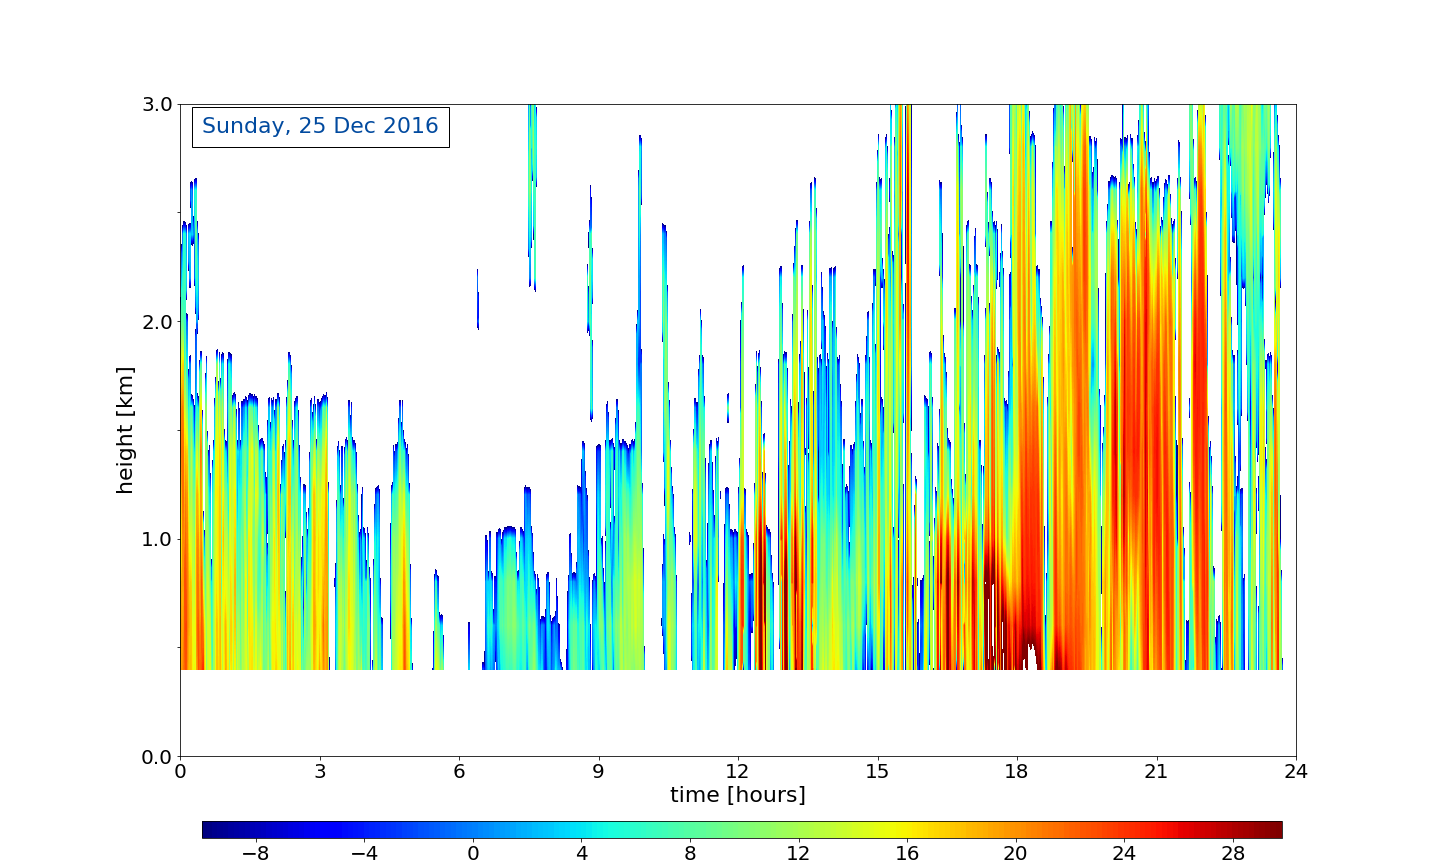
\includegraphics[width=0.6\textwidth]{./fig_MRR/MRR_20161225}
	\caption{Surface temperature at Haukeliseter every minute, for  \SI{25}{\dec}.}\label{fig:MRR_refl}
\end{figure}
% %%%%%%%%%%%%%%%%%%%%%%%%%%%%%%%%%%%%%%%%%%%%%%%%%%%%%%%%%%%%%%%%%%%%%%%%%%
% Observations from the MRR ($y$) are used in \Cref{eq:scalar_cost_fct}.
% 

% Finding a relationship between reflectivity and particle size, common PSD's are used. In the here presented snowfall retrieval an exponential size distribution is assumed (\Cref{eq:PSD}). Attention should be paid, that here snowfall is estimated, where most retrievals use rain. Relationships between reflectivity and snowfall have been developed. Even if the distribution is known, different crystal shapes lead to different results. Furthermore, vary snow density significantly from storm to storm, where small particles are still Rayleigh scattered, and larger particles non-Rayleigh scattered \citep{gunn_microwave_1954}. 

% Only from \Cref{fig:MRR_refl} and \Cref{tab:ref_values} one can not estimate, if snow or rain was present on \SI{25}{\dec}.





% \subsection*{Scattering model}
% $F$, forward model in \Cref{eq:scalar_cost_fct}.
% \subsection*{Final result}
% Snowfall retrieval.

% % #####
% \section{Retrieved Data processing}
% \subsection*{Snow water content}
% To get a valid comparison between the snow water content (SWC) from the optimal estimation retrieval to the MEPS result the SWC is averaged over each hour. MEPS has output values at \SI{0}{}, \SI{1}{}, \SI{2}{}, ..., \SI{22}{}, \SI{23}{\UTC}. To approach the mean values of SWC in the retrieval \SI{30}{\minute} from the previous day and \SI{29}{\minute} from the next day are connected to the array. This leads to a match of the average value at the same time as from MEPS.


% % #####
% \subsection*{Snow water path}
% The snow water path (SWP) of each ensemble member is calculated by using the Simpson's integration rule.  \textcolor{red}{Find reference for equation}
% \begin{align}
% 	\int_{h_0}^{h_1=\SI{3000}{\metre}} SWC(h) \, dh \approx \frac{h_1 - h_0}{6} \left[SWC(h_0) + 4SWC\left(\frac{h_0 + h1}{2}\right) + SWC(h_1) \right] \qquad [\SI{}{\g\per\square\meter}]
%     \label{eq:SWP}
% \end{align}



